\chapter{Introduction}
\label{chp_1_introduction}

Deep Neural Networks (DNNs), one of the most significant models of Artificial Intelligence (AI), have attracted the attention of the whole world. DNNs have revolutionized various domains, such as medical biology \cite{zitnik2019machine}, renewable energy \cite{gensler2016deep}, and autonomous cars \cite{tian2018deeptest}, by enabling complex and intelligent tasks that were previously impossible or impractical. To achieve excellent performance, DNNs must rely highly on enormous matrix multiplications, which require colossal computation power. Conventional processors designed for general-purpose computing cannot meet this demand efficiently, resulting in high energy consumption, long execution time, and limited scalability. Therefore, hardware producers propose a kind of domain-specific hardware called AI processors \cite{Dojo, DBLP:conf/isca/JouppiK0MNNPSST23, Mi300, H100, DBLP:conf/isscc/OuyangDML21, DBLP:conf/hotchips/LiaoTXZ19, 910}, featuring specialized AI acceleration units. Most AI acceleration units target to accelerate the matrix multiplications, named the matrix multiplier-accumulators (MACs). By significantly reducing the execution time of matrix multiplications, the novel hardware naturally improves the performance of the DNNs. 

In addition to the matrix multiplications, the complete AI applications also contain other algorithms and operations, such as the Top-K algorithm in the K-Nearest Neighbors (KNN) \cite{1053964} or Taylor expansion in DNNs \cite{DBLP:conf/cvpr/JinYWMH23}. Compared with matrix multiplications, AI processors have weaker hardware support for scalar or vector operations in 1) quantity, e.g., one 256-bit Vector Unit per core of Huawei Ascend processors \cite{DBLP:conf/hotchips/LiaoTXZ19}; 2) computation power, e.g., 22 TFlops of FP32 vectorized units compared with 362 TFlops of BF16/CFP8 Matrix MACs of Tesla Dojo \cite{Dojo}; and 3) microarchitecture, e.g., removing all sophisticated microarchitectural features, including branch prediction, speculative prefetching, caches, and address coalescing on TPUs \cite{DBLP:conf/isca/JouppiYPPABBBBB17}. The AI processors' specific design and tradeoffs significantly influence the optimization of algorithms. Therefore, a clear understanding of the hardware structure and performance is needed. Taking Huawei Ascend processors \cite{DBLP:conf/hotchips/LiaoTXZ19} as an example, this thesis deeply investigates its architecture and proposes detailed hardware-aware algorithm optimization approaches.

Ascend \cite{DBLP:conf/hotchips/LiaoTXZ19} is a novel hardware architecture provided by Huawei. Based on Ascend architecture, Huawei released Ascend 310 processors for edge devices \cite{DBLP:conf/hotchips/LiaoTXZ19} and Ascend 910B processors for data center servers \cite{910}. Both versions of the processors equip DaVinci Core, which provides 4 TFLOPS (FP16) computation power for matrix multiplication per core. Recently, Huawei introduced a full-stack framework called CANN \cite{CANN}. It allows programmers to design and implement custom DNN operators on the Ascend processors, enabling researchers to propose specific algorithms and optimize their applications \cite{DBLP:conf/ipps/RohwedderCAACW21, DBLP:conf/icpp/JiW21}. However, the novel hardware makes optimizations challenging without a proper performance model that reveals working details and performance implications.

Therefore, this thesis first proposes a performance model of Huawei Ascend AI processor's DaVinci Core, Verrocchio. Given a kernel program of Ascend Cube-based Compute Engine (CCE) instructions, Verrocchio predicts the execution time of each instruction and the whole kernel program based on the discrete-event simulation. To formulate the performance model, in addition to the regular benchmarks for individual hardware unit performance, we develop micro-benchmarks to reveal the bandwidth contention details of the data paths. As a result, the performance model and benchmark results reveal the most critical design tradeoff of the AI processors, intentionally enhancing the Matrix MACs by reducing the support for other necessary operations, including IO, vectorized, and scalar operations. Since complete applications require diverse operations instead of matrix multiplications alone, these inadequate operations significantly slow down overall performance, especially for those non-DNN applications people are trying to adapt.

Considering the specific hardware features, we propose two major approaches to achieve hardware-aware algorithm optimization on the AI processors. The first approach is replacing the most inefficient scalar and vectorized operations with other scalar and vectorized operations. Our benchmarks report that all the scalar operations show similar inefficient performance, while vectorized comparisons \& selections perform the worst among all the operations. Therefore, to illustrate this approach, we present SelB-\textit{k}-NN, a \textit{k}-nearest neighbors algorithm that minimizes the use of these weak operations. The second approach is to map the scalar or vectorized operations onto the Matrix MACs in terms of the matrix multiplications. We demonstrate this approach with Cube-fx, a data layout mapping algorithm that parallelizes Taylor expansion for multiple functions on the Matrix MACs. Although the second approach achieves high performance by activating idle hardware units, not all algorithms can be mapped onto the Matrix MACs. Therefore, we believe both approaches are essential and valuable in the hardware-aware algorithm optimization of AI processors.


\section{Background}
\label{sec_1_1_background}

\subsection{AI Processors}

\begin{sidewaystable}[tbp]
    \caption{Specifications of current popular AI processors}
    \label{tab:sec_1_1_table_1}
    \begin{center}
    
    \scalebox{0.7}{
        \begin{tabular}{c|c|c|c|c}
        \toprule[1pt]
            \textbf{AI Processor} &
            \textbf{\makecell[c]{Exec. \\ Model}} &
            \textbf{Memory Hierarchy} &
            \textbf{AI Acceleration Unit} &
            \textbf{Other Computation Unit} \\
        \midrule[0.5pt]
    
        \makecell[c]{Qualcomm \\ Hexagon 780 \cite{HDSP}} &
        \makecell[c]{SIMT} &
        \makecell[c]{Seamless shared memory for \\ all acceleration units} &
        \multicolumn{2}{|c}{Fused AI Accelerator including Scalar, Tensor \& Vector}
        \\
        \midrule[0.5pt]
    
        \makecell[c]{Google \\ TPU V4 \cite{DBLP:conf/isca/JouppiYPPABBBBB17}} &
        \makecell[c]{SIMD} & 
        \makecell[c]{Unified buffer as local storage \\ DRAM Chips as weights inputs} &
        \makecell[c]{Four ($128 \times 128$) Matrix Multiply Units \\ SparseCore (composed by specific VPUs)} &
        \makecell[c]{128-lane Vector Processing Units \\ No complex microarchitectural features}
        \\
        \midrule[0.5pt]
    
        \makecell[c]{Cambricon \\ MLU290-M5 \cite{MLU290}} &
        \makecell[c]{SIMD} &
        \makecell[c]{Scratchpad memories for units \\ separately w/ DMA to IO} &
        \makecell[c]{Neural Functional Units \\ succeeding to DianNao \cite{DBLP:journals/cacm/ChenCXST16}} &
        \makecell[c]{Unrevealed}
        \\
        \midrule[0.5pt]
    
        \makecell[c]{Nvidia H100 \\ GPU \cite{H100}} &
        \makecell[c]{SIMT} &
        \makecell[c]{GPU memory hierarchy w/ \\ Tensor Core register files} &
        \makecell[c]{640 (16 $\times$ 16 $\times$ 16) Tensor Cores \\ (support sparse matrix)} &
        \makecell[c]{18,432 CUDA cores \\ 80 Streaming Multiprocessors (SMs)}
        \\
        \midrule[0.5pt]
    
        \makecell[c]{Baidu \\ Kunlun K200 \cite{DBLP:conf/isscc/OuyangDML21}} &
        \makecell[c]{SIMD} &
        \makecell[c]{Separate buffers for inputs, and \\ outputs after activation units} &
        \makecell[c]{One MAC array with \\ activation and element-wise units} &
        \makecell[c]{Scalar ALU, Special Function Unit \\ (log, exp, etc.), 256b vector unit}
        \\
        \midrule[0.5pt]
    
        \makecell[c]{Huawei \\ Ascend \cite{DBLP:conf/hotchips/LiaoTXZ19}} &
        \makecell[c]{SIMD} &
        \makecell[c]{Separate L1, L0 buffers for Cube \\ Unit, Unified Buffer for others} &
        \makecell[c]{Cube Unit based on 16 $\times$ 16 \\ tree-like MACs} &
        \makecell[c]{256-bit Vector Unit per core, Scalar \\ Unit for addressing and basic arithmetic}
        \\
    
        \bottomrule[1pt]
        \end{tabular}
    }
    
    \end{center}
    \end{sidewaystable}

AI applications have expanded rapidly in various domains, e.g., natural language generation with GPT-3 \cite{DBLP:conf/nips/BrownMRSKDNSSAA20}, GPT-4 \cite{DBLP:journals/corr/abs-2303-08774}, Llama 2 \cite{DBLP:journals/corr/abs-2307-09288} and image generation with Stable Diffusion \cite{DBLP:conf/cvpr/RombachBLEO22}, Midjourney \cite{DBLP:conf/mindtrek/Oppenlaender22a}, DALL·E 3 \cite{DALLE}. Beneath the fantastic performance of those applications, AI applications heavily rely on elementary matrix multiplications, which demand massive computation power. To meet the requirement, hardware manufacturers have developed AI processors that equip specialized AI acceleration units (\textit{Matrix MACs} in this thesis) for matrix multiplications. 

As shown in Table \ref{tab:sec_1_1_table_1}, we list the hardware details of several popular AI processors. While GPU manufacturers like Nvidia or Qualcomm utilize Single Instruction Multiple Threads (SIMT) to extend their mature GPU architectures, other AI processor manufacturers design their AI processors based on the parallelism of SIMD. Compared with the SIMT execution model, the SIMD model saves power consumption and reduces the hardware scale but loses programming flexibility. The memory hierarchy of the AI processors is generally divided into shared and separate memories. The shared memories aim to decrease the data transfer costs among hardware units, and the separate memories feature different bandwidths and sizes for specific usages. 

The designs of the Matrix MACs vary a lot. Generally, Matrix MACs have a special measurement as a shape, e.g., $(8 \times 8 \times 4)$ for Tesla Dojo, which refers to the shape of the basic matrix multiplication that the Matrix MACs finish in one step, usually in 100 cycles \cite{Mi300}. Then, with accumulators, the Matrix MACs complete the whole matrix multiplication following the law of block matrix multiplication. Most AI processors in the table choose a mini size of the Matrix MACs, like $(16 \times 16 \times 16)$, trying to avoid the low Matrix MACs utilization rates in neural networks \cite{DBLP:conf/hotchips/LiaoTXZ19}, except for Google TPU V4. Since a tiny size of the systolic array would add more loop iterations to the workload and increase the design complexity of the systolic array \cite{DBLP:journals/csur/XuMGL24}, Google chooses a larger shape of $(128 \times 128)$ for their TPUs. 

For other computation units, since Nvidia and AMD GPU designers target to continue growing their mature parallel computation ecosystem, their GPUs still contain a vast number of compute units for massive parallelism in addition to the Matrix MACs. Meanwhile, other designers are trying to lighten the cost of other units to leave more resources for the Matrix MACs. Compared with the GPUs, those AI processors mostly equip only one or two SIMD vectorized units with several scalar units, which provide necessary but limited computation power.

\subsection{Huawei Ascend Processors}
\label{Sec:1_1_2}

The Huawei Ascend architecture draws on the strengths of others with its improvements based on the SIMD execution with a powerful Cube Unit, the Matrix MAC. The DaVinci Core of Huawei Ascend processors has several separate memory buffers supporting the Cube Unit and a shared Unified Buffer for other units. Multiple hardware components constitute DaVinci Core, including compute, storage, and control units. Fig. \ref{fig:dav} illustrates the logic diagrams of Huawei Ascend 310 and 910B AI processors and Fig. \ref{fig:a310} illustrates the hardware structure of an Ascend 310 processor.

\begin{figure}[tb]
    \centering{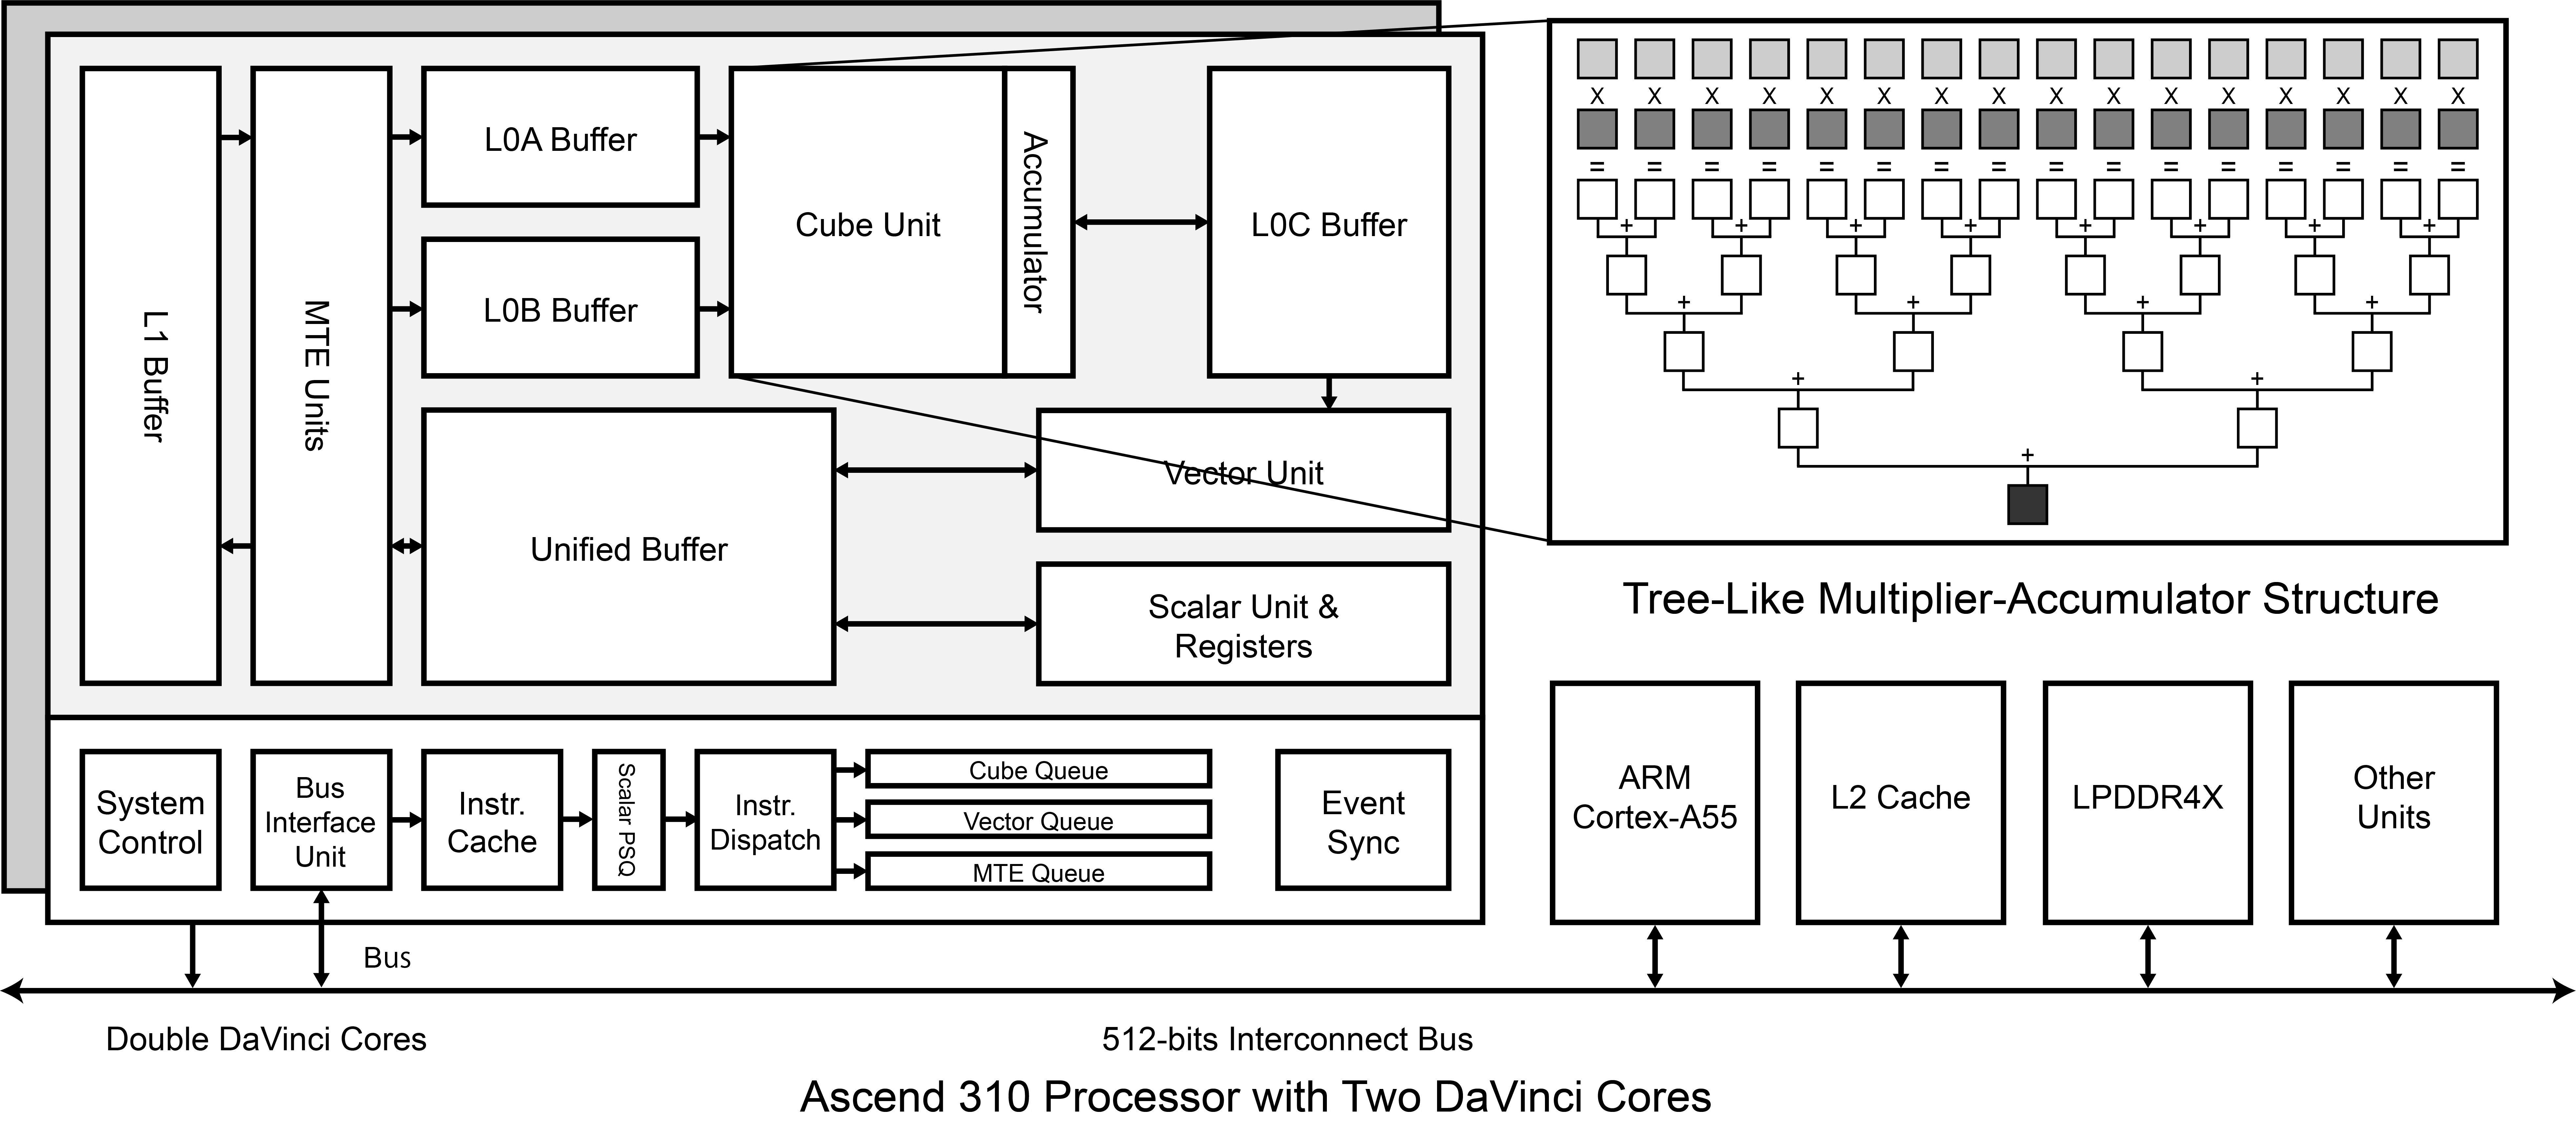
\includegraphics[scale=0.20]{figures/davinci_sub.png}}
    \caption{The hardware structure of an Ascend 310 processor}
    \label{fig:a310}
    \end{figure}

The compute units include the Scalar Unit, Vector Unit, and Cube Unit. The Scalar Unit does mainly address calculations or condition branch analyses. The Vector Unit supports vectorized arithmetic or logical computations, including data preprocessing and activations. The Cube Unit is the essence of the DaVinci Core, improving the computation power of the matrix multiplications. A Cube Unit comprises 4096 FP16 MACs and 8192 INT8 MACs, forming $16 \times 16$ tree-like multiplier-accumulators, as shown in Fig. \ref{fig:a310}. Each matrix multiplication is broken into multiple basic units of $16 \times 16 \times 16$ matrix multiplications. The accumulator behind the Cube Unit accumulates the intermediate results in the L0C Buffer.

The storage units refer to external storage, internal storage, and memory transfer units. The external storage includes L2 Buffer, DDR, and other storage devices accessed by the bus. The internal storage includes five memory buffers (L1, L0A, L0B, L0C, Unified Buffer) and registers. The Memory Transfer Engines (MTEs) control the data paths, which connect the internal storage buffers and transfer the data. The four MTEs (MTE1, MTE2, MTE3, and PIPE\_FIX only for Ascend 910B) are independently tasked with distinct data paths. The five buffers and registers have different capacities and bandwidths, filling the gap between the low bandwidth and the high compute speed. 
        
The control units contain System Control, Scalar Program Scheduling Queue (PSQ), Instruction Dispatch, instruction queues (Cube Queue, Vector Queue, and three MTE Queues), and Event Synchronization. The Scalar PSQ receives and decodes the executing instructions from the Instruction Cache. After decoding, the Instruction Dispatch transmits the instructions to the queues separately. The Event Synchronization handles the data dependency among the units to ensure the correctness of execution orders, mainly a binary semaphore mechanism with eight registers. 

\begin{figure}[tb]
    \centering{\includegraphics[scale=0.25]{figures/ascend.png}}
    \caption{The logic diagrams of Huawei Ascend 310 and 910B hardware structure}
    \label{fig:dav}
    \end{figure}

For the differences in hardware structure, the most significant one is how the Cube Units connect with Vector Units. Fig. \ref{fig:dav} (a) illustrates the structure of Ascend 310, which shows that the major connection is the data path between L0C Buffer and Unified Buffer to transfer the computation results of the Cube Units for the following computation by Vector Units. Meanwhile, Ascend 910B has no direct data path between the two computation units. Instead, Cube Units and Vector Units must read from and write to the global memory, which decouples the computation units. As a result, Ascend 910B processors are constituted by one Cube Core with multiple Vector Cores, as shown in Fig. \ref{fig:dav} (b). Then, the structure changes the one-to-one mapping (one Cube Unit to one Vector Unit) on Ascend 310 to the one-to-many (one Cube Unit to many Vector Units) mapping on Ascend 910B. To quantify the computation power proportion of the Cube Units, we propose CubeRate, which is the throughput rates computed as $Tp_{cube} / (Tp_{cube} + Tp_{vec} + Tp_{scalar})$. Then, the CubeRate of Ascend 310 is $0.95$, and that of Ascend 910B with two Vector Cores is $0.90$, which suggests that the Cube Unit on Ascend 310 is more dominant than that of Ascend 910B. In addition, Ascend 910B processors need a slow inter-core binary semaphore supported by the slow global memory to synchronize the Cube Units and Vector Units. In contrast, Ascend 310 processors only require the intra-core binary semaphore supported by registers. Therefore, on Ascend 910B processors, although one Cube Unit has multiple Vector Units for supporting, the data communication costs between the Cube Units and Vector Units are highly increased, potentially weakening the advantages brought by the cooperation. 

\subsection{Dissection and Optimization on AI processors}
\label{Sec:1_1_3}

With the growth of the AI processors, researchers paid high interest in this novel hardware with a lot of work in different areas. Similar to the previous works on regular GPUs \cite{DBLP:conf/ppopp/ZhangTXLZC17}, researchers have launched dissection works on the AI processors, e.g., the architecture of the Tensor Cores \cite{DBLP:journals/corr/abs-1804-06826}. Therefore, based on these dissections, some studies have been working on performance modeling on the AI processors. Their models can be divided into two categories: white-box hardware model \cite{DBLP:conf/ispass/RaihanGA19} and black-box statistics model \cite{DBLP:conf/nips/ChenZYJMCGK18, DBLP:journals/corr/abs-2008-01040}. The white-box hardware model requires a deep understanding of the hardware, which makes the model explainable but usually not general. Meanwhile, the black-box statistics model requires no hardware details but large scales of previous execution records for model training. 

In addition, more works focus on the optimization of the AI processors. At the level of the applications, studies focus on optimizing the original tasks of the AI processors, the matrix multiplications \cite{gccblas, oneapi, 9820727, 9139835}. Meanwhile, a vast research direction is to extend the application of the AI processors to general computation. Navarro \textit{et al.} \cite{DBLP:conf/sccc/CarrascoVN18} and Dakkak \textit{et al.} \cite{DBLP:conf/ics/DakkakLXGH19} convert the basic operations of reduction and scan into special matrix multiplications by the Matrix MACs on Nvidia GPUs. Their designs divide the input data into segments of different sizes and then compute the operations from warps to blocks following the CUDA compute hierarchy with Tensor Cores. Tang \textit{et al.} \cite{DBLP:conf/ic-nc/TangK0K20} design a dense matrix multiplication to compute skinny matrix multiplications with Tensor Cores, significantly increasing the Matrix MACs' utilization rate. Lee \textit{et al.} \cite{DBLP:journals/access/LeeSZH22} computes the polynomial convolutions by matrix multiplications for their Lattice-based cryptography with Tensor Cores. Hu \textit{et al.} \cite{10.1145/3514221.3517869} accelerates different types of join operaitons with the matrix MACs. Compared with those previous studies, our Cube-fx also designs special matrix multiplications to enhance the performance of the building and computation of Taylor polynomials, which reports significant improvement.

\section{Motivations}
\label{sec_1_2_motivations}

\subsection{Hidden Hardware Details of AI Processors}

Although hardware manufacturers have published various architectures of AI processors, the public and community are still unfamiliar with the hardware in addition to limited hardware parameters, e.g., FLOPS. These parameters provide a too-general view of the hardware performance instead of helpful information for potential algorithm migration or optimization. One of the reasons for the unfamiliarity is that most AI processors have no physical consumer-grade products but are only available on the cloud. Then, the evaluations offered by the researchers are influenced by the virtual environments and the sharing policies on the cloud, which report inaccurate results and hide the architecture details. Another reason is that the toolchains of most AI processors are usually inadequate and only leave high-level abstraction APIs, primarily as operations in deep learning frameworks. Therefore, programmers cannot implement instruction-level benchmarks for detailed hardware parameters, including bandwidths or throughputs. Table \ref{tab:sec_1_2_table_1} reports the availability and API level of some popular AI processor manufacturers.

\begin{table}[tbp]
    \caption{Availability and API level of AI processor manufacturers}
    \label{tab:sec_1_2_table_1}
    \begin{center}
    
    \scalebox{0.85}{
        \begin{tabular}{c|c|c}
        \toprule[1pt]
            \textbf{Manufacturer} &
            \textbf{\makecell[c]{Public Availability}} &
            \textbf{API Level} \\
        \midrule[0.5pt]
    
        \makecell[c]{Qualcomm} &
        \makecell[c]{Mobile SOC \cite{HDSP}} &
        \makecell[c]{Operations in QNN \cite{QNN}}
        \\
        \midrule[0.5pt]
    
        \makecell[c]{Google} &
        \makecell[c]{Cloud platforms \cite{DBLP:conf/isca/JouppiYPPABBBBB17}} & 
        \makecell[c]{Operations in TensorFlow or \\ PyTorch XLA \cite{XLA}}
        \\
        \midrule[0.5pt]
    
        \makecell[c]{Cambricon} &
        \makecell[c]{Cloud platforms \cite{DevP}} &
        \makecell[c]{Low-level C \& assembly \cite{BANG}}
        \\
        \midrule[0.5pt]
    
        \makecell[c]{Nvidia} &
        \makecell[c]{Physical cards \cite{ADA}} &
        \makecell[c]{Low-level CUDA \& PTX \cite{PTX}}
        \\
        \midrule[0.5pt]
    
        \makecell[c]{Baidu} &
        \makecell[c]{Internal usage} &
        \makecell[c]{Applications in Baidu AI Cloud \cite{Pad}}
        \\
        \midrule[0.5pt]
    
        \makecell[c]{Huawei} &
        \makecell[c]{Physical cards \cite{DBLP:conf/hotchips/LiaoTXZ19}} &
        \makecell[c]{Low-level C \& assembly \cite{CANN}}
        \\
    
        \bottomrule[1pt]
        \end{tabular}
    }
    
    \end{center}
    \end{table}

In addition to the Nvidia GPUs \cite{DBLP:journals/corr/abs-1804-06826, DBLP:conf/ppopp/ZhangTXLZC17, DBLP:conf/ics/ZhouTZWS17, DBLP:conf/ispass/RaihanGA19, DBLP:conf/pldi/HongSKRKPRS18, DBLP:conf/cgo/ZhouMSM21}, the lack of hardware details of the AI processors brings a significant problem to algorithm migration or optimization. For instance, given a matrix multiplication of $(256 \times 256 \times 256)$, Huawei Ascend processors require more loop iterations to execute matrix MACs than Google TPUs, since the size of the former ($16 \times 16$) is much smaller than that of the latter ($128 \times 128$). Therefore, the optimized tiling parameters of the matrix multiplications should be different. Without the hardware details of the matrix MAC size, programmers would not do such a tiling parameter analysis and face enormous challenges for algorithm optimization. Therefore, this thesis first performs a comprehensive dissection with various benchmarks on the Huawei Ascend AI processor to reveal its hardware details.

\subsection{Inefficient Hardware Units on AI Processors \label{sec_1_2_2}}

\begin{figure}[tbp]
    \centering{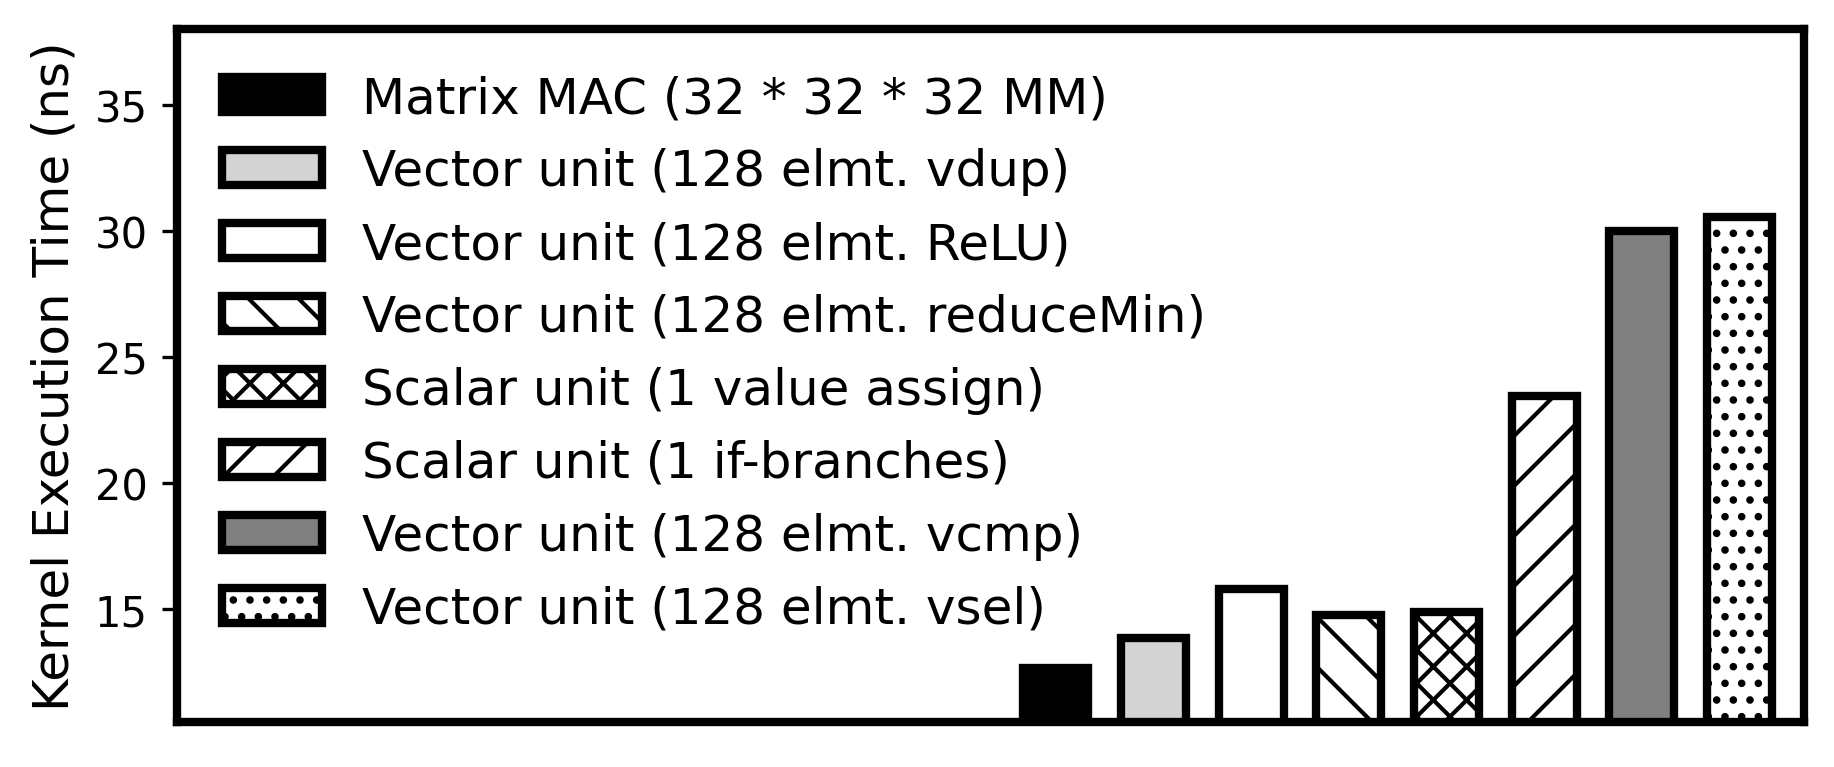
\includegraphics[scale=0.7]{figures/background_data.png}}
    \caption{The benchmark results on Huawei Ascend 310 AI processors}
    \label{fig:benchmark}
    \end{figure}

As independent processors, the AI processors are equipped with additional units other than the Matrix MACs for necessary operations, including instruction dispatching or vectorized computation. As discussed and listed in Table \ref{tab:sec_1_1_table_1}, except for GPUs, designers usually prefer assigning more hardware resources to enhance the performance of the matrix multiplications. 

On the Huawei Ascend 310 AI processor, we offer an instruction-level benchmark, where each test contains variable numbers of manually duplicated operations, e.g., $(32 \times 32 \times 32)$ matrix multiplication for the Matrix MACs, $128$ ReLU for the vector units, and $1$ if-branching for the scalar units. By raising the number of executed operations, we collect the increased execution time as the execution time of every single instruction. Fig. \ref{fig:benchmark} shows that a scalar single-operand conditional branch (if-branching) takes an average of 1.48$\times$ longer than \verb|ReLU|, 1.69$\times$ longer than \verb|vecDup|, 1.60$\times$ longer than \verb|reduceMin| on 128 elements in parallel. An immediate assignment to on-core memory takes 0.94$\times$ of \verb|ReLU|, where \verb|ReLU| consists of data reading, computation, and data writing. The vectorized comparisons \& selections take 1.90$\times$ and 1.93$\times$ than \verb|ReLU| respectively, showing lower efficiency. The hardware features restrict the migrations of classical algorithms from other platforms. Even after successful migrations, the implementations could face heavy performance loss.

\subsection{Low Usage Rate of Matrix MACs}

Since the Matrix MACs of the AI processors compute matrix multiplications only, most algorithms or applications cannot utilize the high-performance Matrix MACs. Even for the algorithms containing matrix multiplications, the usage rate of the Matrix MACs is still far lower than expected.

\begin{figure}[tbp]
    \centering{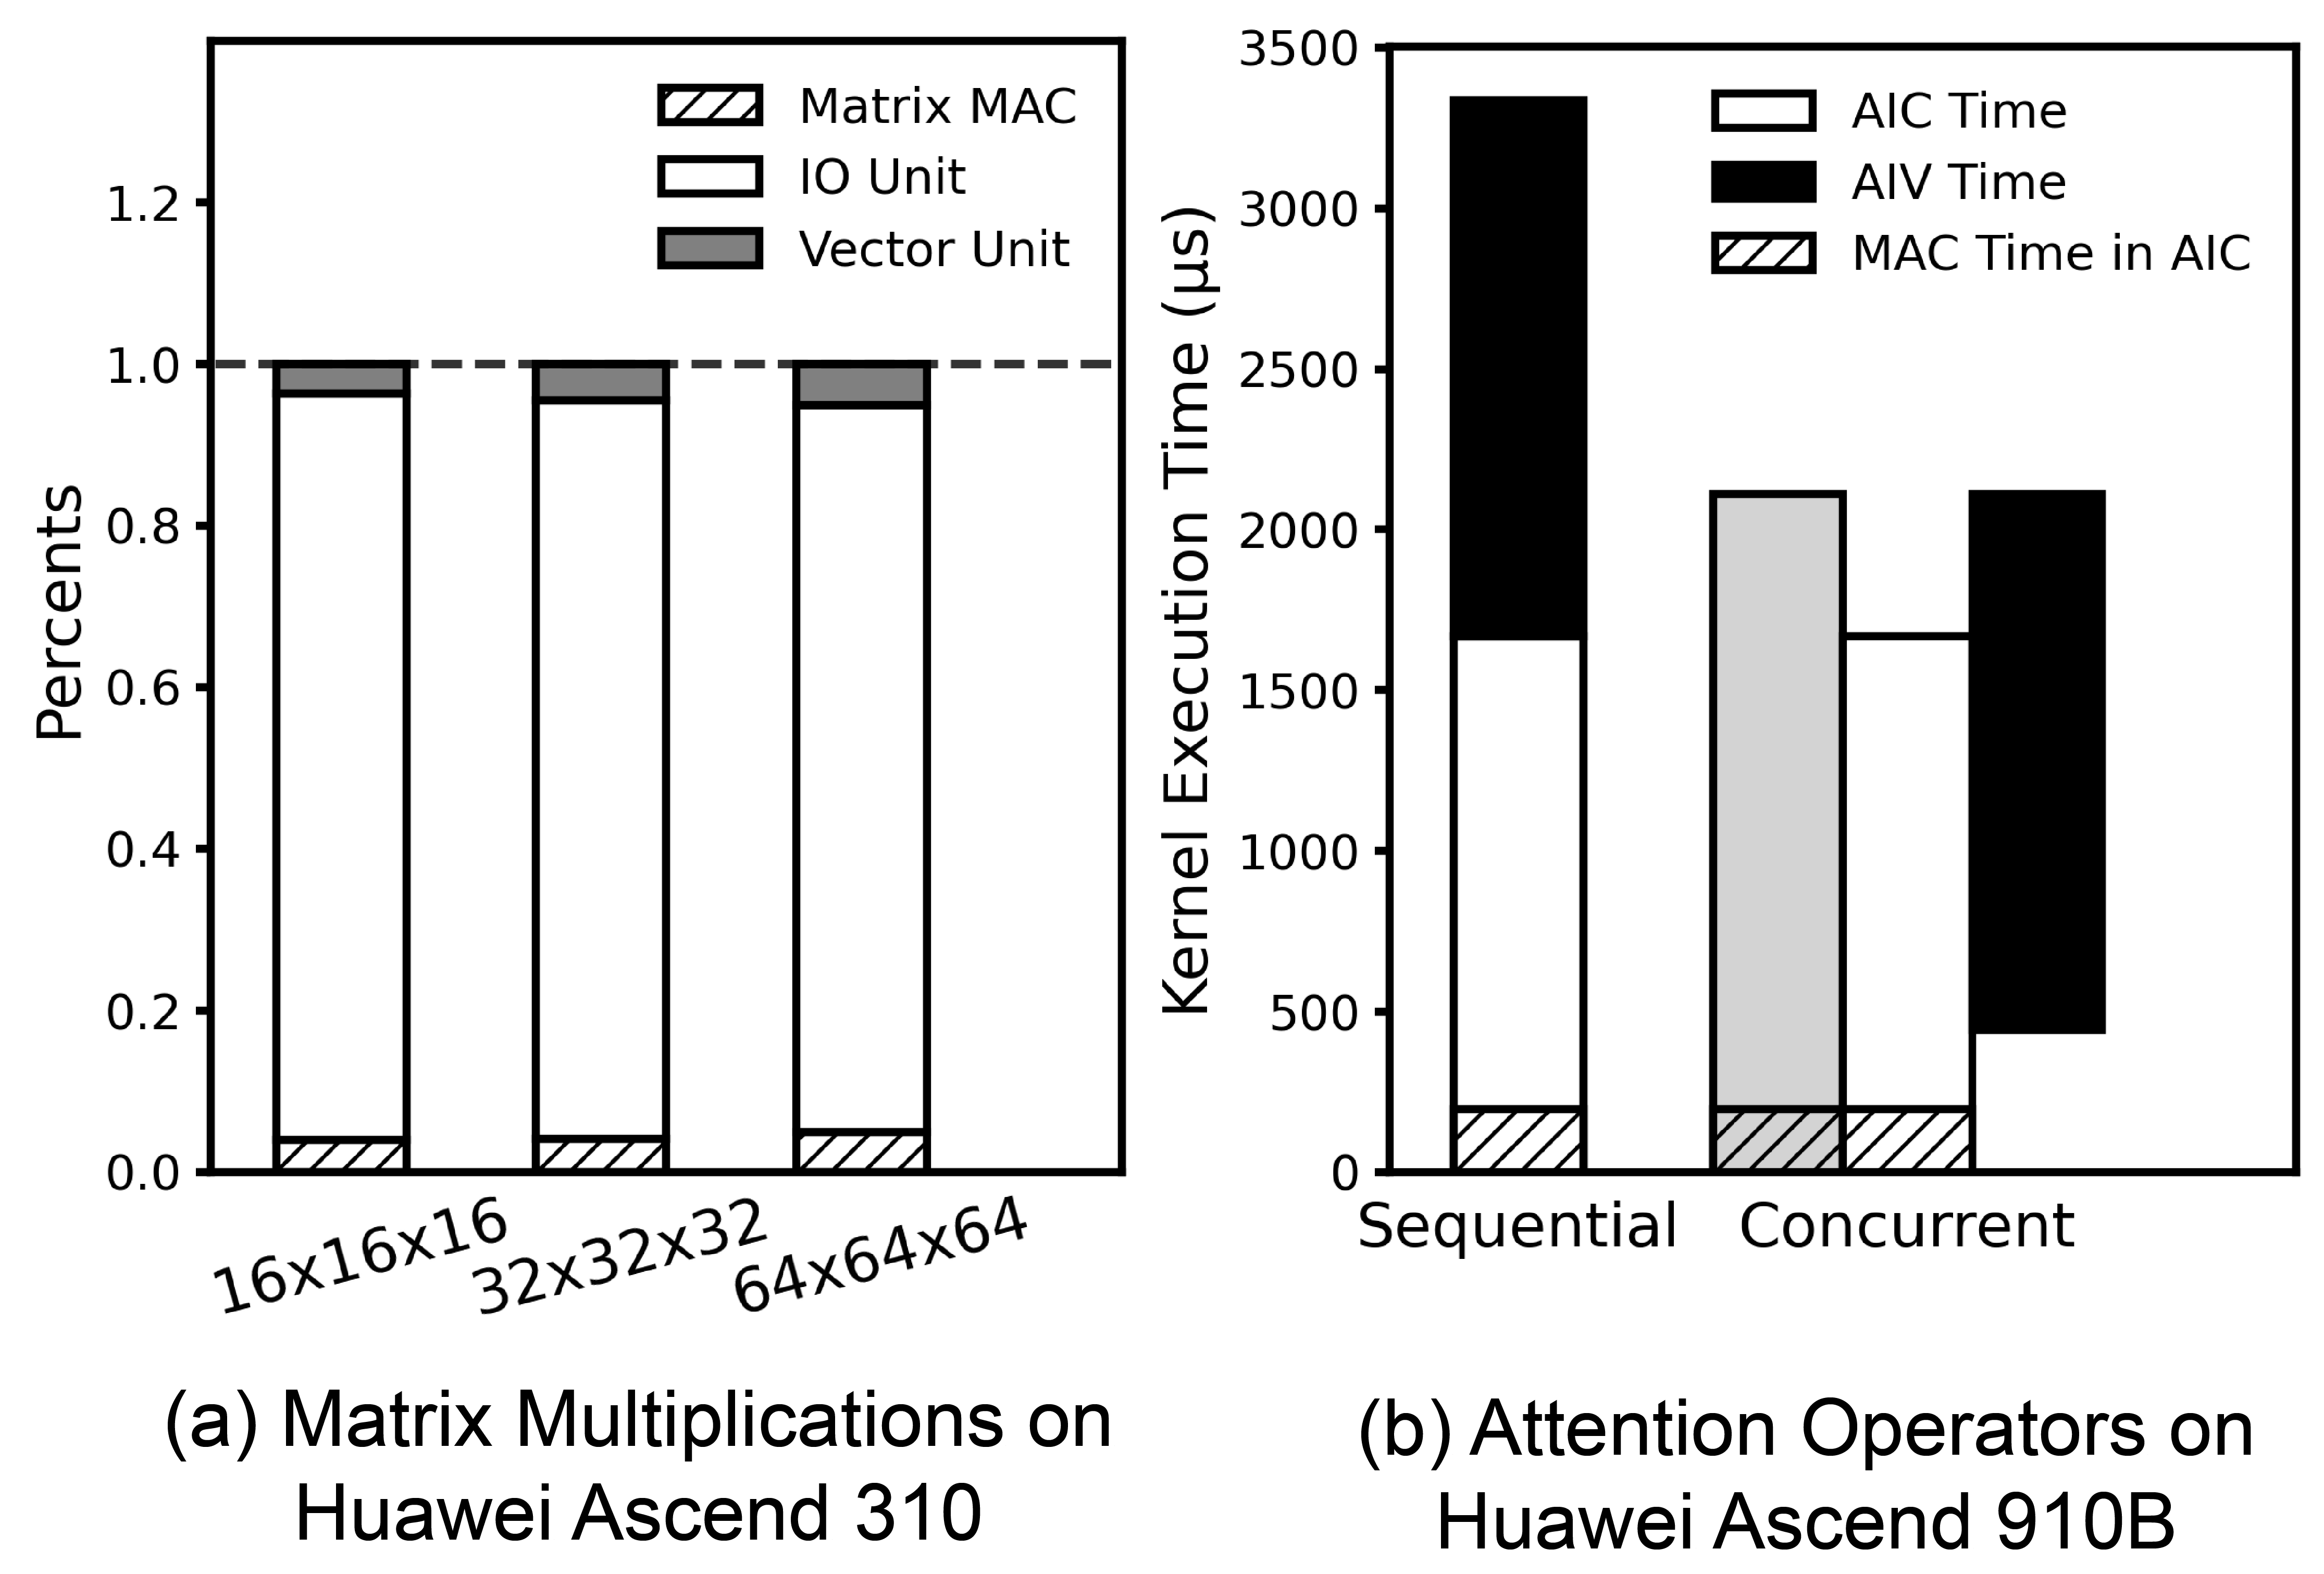
\includegraphics[scale=0.25]{figures/background_flash.png}}
    \caption{The percents of matrix multiplication rates on Ascend 310 and 910B processors}
    \label{fig:back_flash}
    \end{figure}

Former studies and official documents \cite{moustafaaccelerating, cann_sugg} have discussed the low usage of the Cube Units and weak performance of the Vector Units in Ascend 310. Furthermore, we pick two representative applications on Ascend 310 and Ascend 910B: matrix multiplications and attention \cite{DBLP:conf/nips/VaswaniSPUJGKP17}. Fig. \ref{fig:back_flash} (a) reports the evaluation results of matrix multiplications on Ascend 310, where we can observe a shallow usage rate of Matrix MACs (less than 5$\%$). The evaluation results on Ascend 910B are more complicated. The execution time of the Cube Units (Cube Core) and Vector Units (Vector Cores) are counted separately as AIC Time and AIV Time. Therefore, the AIC Time in Fig. \ref{fig:back_flash} (b) reports the execution time of pure matrix multiplications, the same as the matrix multiplications on Ascend 310. Even though the implementation of attention operators contains massive $(128 \times 128 \times 128)$ and $(256 \times 128 \times 256)$ matrix multiplications, in both naive sequential and highly optimized concurrent execution, the usage rate of Matrix MACs is still low. The evaluation results suggest that on both versions of Ascend processors, the low usage of Matrix MACs remains a significant problem, allowing us to implement more efficient algorithms with the cooperation of both units.

\section{Main contributions}
\label{sec_1_3_contributions}

\subsection{Performance Modeling on Huawei Ascend}

We first demystify the Huawei Ascend 310 with micro-benchmarks to show the characteristics of the hardware units on DaVinci Core, the AI Core of the Huawei Ascend processor. We pay the most attention to the IO units, which play the most critical role and influence the execution time. We reveal how MTE Units control and compete for the data paths that connect the different separate memories. In addition to the contention ratio benchmark on bandwidth sharing, we design specially-crafted benchmarks to identify the source, which is asserted to be the Interconnect Bus, and the runtime behaviors of the bus contention.

Then, we propose a discrete-event-based performance model, \textbf{Verrocchio}. Verrocchio models a series of architectural features that are most important and determinant for the DaVinci Core performance, including bandwidth contentions and concurrent hardware unit execution with synchronization. The evaluation results show that Verrocchio achieves an average error rate of $2.62\%$ and $2.30\%$ for the single-core and double-core execution of several sample kernels. We demonstrate the use of Verrocchio in optimizing a matrix multiplication algorithm. Verrocchio enables a search space exploration in tiling size selection and achieves a speedup of 1.70$\times$ at the operator level and 1.53$\times$ at the application level compared with CANN \cite{CANN} native operators with prediction error rates of $5.06\%$ and $5.25\%$ for the single-core and double-core execution.

\subsection{1) Replacing the Worst Operations}

\textbf{SelB-\textit{k}-NN} (\textbf{Sel}ection-\textbf{B}itonic-\textbf{\textit{k}}-\textbf{NN}) is a mini-batch \textit{k}-NN for the powerful AI processors. For a single batch, SelB-\textit{k}-NN includes a naturally-accelerated distance computation and a non-trivial \textit{k}-selection. For the \textit{k}-selection, inspired by the selection sort, SelB-\textit{k}-NN compares the minimized value of the distance computation results with the first element of the min-\textit{k} result array, maintained by the bitonic 1-selection \cite{DBLP:conf/sigmod/ShanbhagPM18}. Compared with the previous approaches, SelB-\textit{k}-NN limits the increment of the weakly-supported scalar operations, vectorized comparisons \& selections. Since the architectures and instruction sets of the AI processors vary among manufacturers, we propose two algorithms to minimize the hardware support requirements for better portability. As a result, only \verb|vecDup|, \verb|ReLU|, and \verb|reduceMin| (\verb|reduceMax|) with no indexing are sufficient, which contribute to the most significant and necessary operators on most AI processors. For all mini-batches, an early exit policy dynamically reduces most of the \textit{k}-selection workloads, which our quantification shows shrink in an inverse proportion. We model the tiling shape selection to an optimization problem, considering the overall performance of SelB-\textit{k}-NN. In addition, we propose an offline pruning method working during preprocessing to reduce the optimization problem's search space.

\subsection{2) Transforming to Matrix Multiplications}

\textbf{Cube-}$\mathbf{fx}$ is a data layout mapping that parallelizes Taylor expansion for function evaluation by leveraging the computational power of the Matrix MACs. With one other matrix containing a row of an ascending sequence, Cube-fx expresses the building and computation of Taylor polynomials in terms of a pair of two matrix multiplications. Cube-fx has two stages: preparation and computation. The preparation stage focuses on reformatting the data layout of the inputs. Since the variables of the Taylor polynomials are several vectors $(x^{k_0}, x^{k_1}, x^{k_2}, ...)$ contiguously listed in the L0 Buffers, Cube-fx first scatters a batch of inputs and constructs the corresponding vectors in the preparation stage. Then, Cube-fx evaluates multiple independent functions in the computation stage by reusing the vectors generated by the preparation stage with different coefficients in parallel. Depending on different precision requirements, Cube-fx applies a required order of expansion to approximate the original functions. When given a low order requirement, Cube-fx achieves higher data parallelism with a further data layout mapping algorithm. With the direct sums of the input and coefficient matrices of Cube-fx, the mapping helps Cube-fx to condense the matrix multiplications and compute multiple inputs within one basic matrix multiplication. Furthermore, when the total length of multiple input vectors is larger than the side length of the Matrix MACs, multiple basic matrix multiplications are required by Cube-fx. By counting the number of basic matrix multiplications as a new metric, Matrix MAC Count, we formulate an optimization problem to find the best number of merged input vectors to minimize the Matrix MAC Count and data movement. Compared with previous approaches, Cube-fx significantly reduces the vector operations, which perform weakly on the AI processors, reuses the intermediate results, and migrates most of the computation to the Matrix MACs by doing special cases of matrix multiplications. Cube-fx can be implemented on most AI processors, which performs more efficiently for those devices with limited vectorized units and high-speed communication between the vectorized units and Matrix MACs.

\section{Thesis Organization}
\label{sec_1_4_organization}

The rest of this thesis is organized as follows. Chapter 2 starts with demystifying and benchmarking the Huawei Ascend AI processors. Then, it introduces a performance model, Verrocchio, and gives complete evaluations for its accuracy. Chapter 3 discusses the first optimization approach, replacing the most inefficient scalar or vectorized operations with others. Chapter 4 discusses the second optimization approach, replacing the vectorized and scalar operations with specific matrix multiplications. Chapter 5 concludes this thesis and suggests possible future works.